\documentclass{article}
\usepackage[utf8]{inputenc}
\usepackage[left=2cm, right=2cm]{geometry}
\title{Szemerédi Regularity Lemma}

\author{Aakash Ghosh(19MS129)}

%\date{28 March 2010} % without \date command, current date is supplied

%\geometry{showframe} % display margins for debugging page layout


\usepackage{amsmath}  % extended mathematics
\usepackage{booktabs} % book-quality tables
\usepackage{units}    % non-stacked fractions and better unit spacing
\usepackage{multicol} % multiple column layout facilities
\usepackage{lipsum}   % filler text
\usepackage{fancyvrb} % extended verbatim environments
	\fvset{fontsize=\normalsize}% default font size for fancy-verbatim environments
\usepackage{amsthm}

\newtheorem{theorem}{Theorem}[]
\newtheorem{definition}{Definition}[]
\newtheorem{corollary}{Corollary}[theorem]
\newtheorem{lemma}[theorem]{Lemma}

\setcounter{secnumdepth}{-1}

\usepackage{physics}
\usepackage{amsmath}
\usepackage{tikz}
\usepackage{mathdots}
\usepackage{yhmath}
\usepackage{cancel}
\usepackage{color}
\usepackage{array}
\usepackage{multirow}
\usepackage{amssymb}
\usepackage{gensymb}
\usepackage{tabularx}
\usepackage{extarrows}
\usepackage{booktabs}
\usetikzlibrary{fadings}
\usetikzlibrary{patterns}
\usetikzlibrary{shadows.blur}
\usetikzlibrary{shapes}

\begin{document}

\maketitle

\noindent
Let $G$ be a graph and let $A$ and $B$ be disjoint set of vertices of $G$ and let $e_GA,B)$ be the number of edges from $A$ to $B$ in $G$. Define a density function $d(A,B)=\frac{e_GA,B)}{|A||B|}$\\
\textbf{Remark: }Note that $d(A,B)$ is a somewhat normalised measure of how well two vertex set is connected  with each other. The value of $d$ will range from 0(i.e no connection) to 1(i.e. all possible edges are present and very well-connected)


\begin{lemma}
	If $y\in[a,b]$ then
	\begin{align}
	|x-y|\leq  c\forall y\in[a,b]\Leftrightarrow |x-a|\leq  c,|x-b|\leq  c
	\end{align}
\end{lemma}
\begin{proof}
There are three possible cases as shown in Fig 1. The blue line shows the values $y$ takes.
\begin{figure}
\centering

	\tikzset{every picture/.style={line width=0.75pt}} %set default line width to 0.75pt

	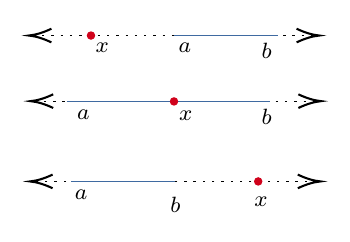
\begin{tikzpicture}[x=0.75pt,y=0.75pt,yscale=-1,xscale=1]
	%uncomment if require: \path (0,300); %set diagram left start at 0, and has height of 300

	%Straight Lines [id:da44850145401460706]
	\draw  [dash pattern={on 0.84pt off 2.51pt}]  (92.86,81.61) -- (228.86,81.61) ;
	\draw [shift={(230.86,81.61)}, rotate = 180] [color={rgb, 255:red, 0; green, 0; blue, 0 }  ][line width=0.75]    (10.93,-3.29) .. controls (6.95,-1.4) and (3.31,-0.3) .. (0,0) .. controls (3.31,0.3) and (6.95,1.4) .. (10.93,3.29)   ;
	\draw [shift={(90.86,81.61)}, rotate = 0] [color={rgb, 255:red, 0; green, 0; blue, 0 }  ][line width=0.75]    (10.93,-3.29) .. controls (6.95,-1.4) and (3.31,-0.3) .. (0,0) .. controls (3.31,0.3) and (6.95,1.4) .. (10.93,3.29)   ;
	%Straight Lines [id:da44467407695726846]
	\draw [color={rgb, 255:red, 63; green, 106; blue, 161 }  ,draw opacity=1 ]   (108.29,81.61) -- (206.29,81.61) ;
	%Straight Lines [id:da03160934519071412]
	\draw  [dash pattern={on 0.84pt off 2.51pt}]  (92,50) -- (228,50) ;
	\draw [shift={(230,50)}, rotate = 180] [color={rgb, 255:red, 0; green, 0; blue, 0 }  ][line width=0.75]    (10.93,-3.29) .. controls (6.95,-1.4) and (3.31,-0.3) .. (0,0) .. controls (3.31,0.3) and (6.95,1.4) .. (10.93,3.29)   ;
	\draw [shift={(90,50)}, rotate = 0] [color={rgb, 255:red, 0; green, 0; blue, 0 }  ][line width=0.75]    (10.93,-3.29) .. controls (6.95,-1.4) and (3.31,-0.3) .. (0,0) .. controls (3.31,0.3) and (6.95,1.4) .. (10.93,3.29)   ;
	%Shape: Circle [id:dp5333382021730819]
	\draw  [color={rgb, 255:red, 208; green, 2; blue, 27 }  ,draw opacity=1 ][fill={rgb, 255:red, 208; green, 2; blue, 27 }  ,fill opacity=1 ] (118.25,50) .. controls (118.25,49.03) and (119.03,48.25) .. (120,48.25) .. controls (120.97,48.25) and (121.75,49.03) .. (121.75,50) .. controls (121.75,50.97) and (120.97,51.75) .. (120,51.75) .. controls (119.03,51.75) and (118.25,50.97) .. (118.25,50) -- cycle ;
	%Straight Lines [id:da028463898146168343]
	\draw [color={rgb, 255:red, 63; green, 106; blue, 161 }  ,draw opacity=1 ]   (160,50) -- (210,50) ;
	%Shape: Circle [id:dp2813904121246703]
	\draw  [color={rgb, 255:red, 208; green, 2; blue, 27 }  ,draw opacity=1 ][fill={rgb, 255:red, 208; green, 2; blue, 27 }  ,fill opacity=1 ] (158.25,81.75) .. controls (158.25,80.78) and (159.03,80) .. (160,80) .. controls (160.97,80) and (161.75,80.78) .. (161.75,81.75) .. controls (161.75,82.72) and (160.97,83.5) .. (160,83.5) .. controls (159.03,83.5) and (158.25,82.72) .. (158.25,81.75) -- cycle ;
	%Straight Lines [id:da2300956631550083]
	\draw  [dash pattern={on 0.84pt off 2.51pt}]  (228.57,120.29) -- (92.57,120.29) ;
	\draw [shift={(90.57,120.29)}, rotate = 360] [color={rgb, 255:red, 0; green, 0; blue, 0 }  ][line width=0.75]    (10.93,-3.29) .. controls (6.95,-1.4) and (3.31,-0.3) .. (0,0) .. controls (3.31,0.3) and (6.95,1.4) .. (10.93,3.29)   ;
	\draw [shift={(230.57,120.29)}, rotate = 180] [color={rgb, 255:red, 0; green, 0; blue, 0 }  ][line width=0.75]    (10.93,-3.29) .. controls (6.95,-1.4) and (3.31,-0.3) .. (0,0) .. controls (3.31,0.3) and (6.95,1.4) .. (10.93,3.29)   ;
	%Shape: Circle [id:dp9955225061412448]
	\draw  [color={rgb, 255:red, 208; green, 2; blue, 27 }  ,draw opacity=1 ][fill={rgb, 255:red, 208; green, 2; blue, 27 }  ,fill opacity=1 ] (202.32,120.29) .. controls (202.32,121.25) and (201.54,122.04) .. (200.57,122.04) .. controls (199.6,122.04) and (198.82,121.25) .. (198.82,120.29) .. controls (198.82,119.32) and (199.6,118.54) .. (200.57,118.54) .. controls (201.54,118.54) and (202.32,119.32) .. (202.32,120.29) -- cycle ;
	%Straight Lines [id:da44950411402465784]
	\draw [color={rgb, 255:red, 63; green, 106; blue, 161 }  ,draw opacity=1 ]   (160.57,120.29) -- (110.57,120.29) ;


	% Text Node
	\draw (161,52.4) node [anchor=north west][inner sep=0.75pt]  [font=\footnotesize]  {$a$};
	% Text Node
	\draw (201,52.4) node [anchor=north west][inner sep=0.75pt]  [font=\footnotesize]  {$b$};
	% Text Node
	\draw (121,52.4) node [anchor=north west][inner sep=0.75pt]  [font=\footnotesize]  {$x$};
	% Text Node
	\draw (112,84.4) node [anchor=north west][inner sep=0.75pt]  [font=\footnotesize]  {$a$};
	% Text Node
	\draw (201,84.15) node [anchor=north west][inner sep=0.75pt]  [font=\footnotesize]  {$b$};
	% Text Node
	\draw (161.21,85.08) node [anchor=north west][inner sep=0.75pt]  [font=\footnotesize]  {$x$};
	% Text Node
	\draw (111,123.11) node [anchor=north west][inner sep=0.75pt]  [font=\footnotesize]  {$a$};
	% Text Node
	\draw (157,126.44) node [anchor=north west][inner sep=0.75pt]  [font=\footnotesize]  {$b$};
	% Text Node
	\draw (197.5,126.65) node [anchor=north west][inner sep=0.75pt]  [font=\footnotesize]  {$x$};


	\end{tikzpicture}
	\caption{The three cases required to prove lemma 1}
\end{figure}
\end{proof}



\begin{theorem}
	If $X\subset A$ and $Y\subset B$ with $\frac{|X|}{|A|}\geq  1-\delta$ and $\frac{|Y|}{|B|}\geq  1-\delta$ where $0\leq  \delta\leq \frac{1}{2}$. Then:
	\begin{align}
	|d(X,Y)-d(A,B)|\leq  2\delta\\
	|d^2(X,Y)-d^2(A,B)|\leq  4\delta
	\end{align}
\end{theorem}
\noindent\textbf{\textit{Proof outline:}} We try to go the other way around: we fix edges of $X,Y$ and try to build edges of $A,B$ around them. We note that since $d(A,B)$ increases with the number of edges added in the extension of the old graph, we just need to make sure that inequality holds for the maximum and minimum values only(lemma 1). We find bounds for this maximum and minimum values to complete the proof. Eqn3 follows as a consequence of Eqn2 and bounds on $d(A,B),d(X,Y)$.
\begin{proof}
	Let $d(X,Y)=d'$. Note that:
	\begin{align}
	e_G(A,B)=e_G(X,Y)+e_G(X,B\setminus Y)+e_G(A\setminus X,Y)+e_G(A\setminus X,B\setminus Y)
	\end{align}
\noindent
We shall first try to prove the inequality when  $d(A,B)=d_1$ is maximum. It is  easy to see this occurs when each term of eqn4 attains their maximum value. Note only $e_G(X,Y)$ is fixed. For the other terms we have:
\begin{figure}
\centering

	\tikzset{every picture/.style={line width=0.75pt}} %set default line width to 0.75pt

	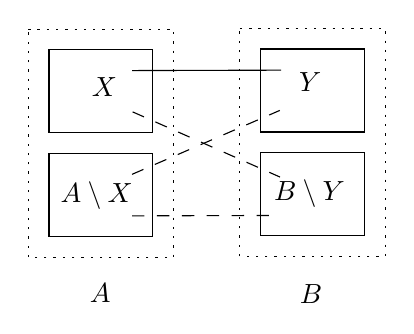
\begin{tikzpicture}[x=0.75pt,y=0.75pt,yscale=-1,xscale=1]
	%uncomment if require: \path (0,300); %set diagram left start at 0, and has height of 300

	%Shape: Rectangle [id:dp6627426419684201]
	\draw  [dash pattern={on 0.84pt off 2.51pt}] (50,60) -- (120,60) -- (120,170) -- (50,170) -- cycle ;
	%Shape: Rectangle [id:dp3761312539244661]
	\draw   (60,70) -- (110,70) -- (110,110) -- (60,110) -- cycle ;
	%Shape: Rectangle [id:dp4675212630222737]
	\draw   (60,120) -- (110,120) -- (110,160) -- (60,160) -- cycle ;
	%Shape: Rectangle [id:dp5057622954470224]
	\draw  [dash pattern={on 0.84pt off 2.51pt}] (152,59.6) -- (222,59.6) -- (222,169.6) -- (152,169.6) -- cycle ;
	%Shape: Rectangle [id:dp43815436760732673]
	\draw   (162,69.6) -- (212,69.6) -- (212,109.6) -- (162,109.6) -- cycle ;
	%Shape: Rectangle [id:dp28652760393509646]
	\draw   (162,119.6) -- (212,119.6) -- (212,159.6) -- (162,159.6) -- cycle ;
	%Straight Lines [id:da24802555849916097]
	\draw    (100,80) -- (171.8,79.8) ;
	%Straight Lines [id:da8218556337757607]
	\draw  [dash pattern={on 4.5pt off 4.5pt}]  (100,150) -- (171.8,149.8) ;
	%Straight Lines [id:da37241741334903355]
	\draw  [dash pattern={on 4.5pt off 4.5pt}]  (100.3,99.9) -- (171.3,131.3) ;
	%Straight Lines [id:da19373579144542075]
	\draw  [dash pattern={on 4.5pt off 4.5pt}]  (100,130) -- (171.2,99.2) ;

	% Text Node
	\draw (79.4,82) node [anchor=north west][inner sep=0.75pt]    {$X$};
	% Text Node
	\draw (64.4,132.4) node [anchor=north west][inner sep=0.75pt]    {$A\setminus X$};
	% Text Node
	\draw (179.2,79.6) node [anchor=north west][inner sep=0.75pt]    {$Y$};
	% Text Node
	\draw (167.2,131.2) node [anchor=north west][inner sep=0.75pt]    {$B\setminus Y$};
	% Text Node
	\draw (78.4,181.6) node [anchor=north west][inner sep=0.75pt]    {$A$};
	% Text Node
	\draw (179.6,182) node [anchor=north west][inner sep=0.75pt]    {$B$};


	\end{tikzpicture}
	\caption{Each line represents all edges between the sets it joins. Edges represented by the solid line is given. Maximum is attained when all edges represented by the dotted line is present. Minimum is attained when no edge of represented by dotted lines are given.}
\end{figure}
\begin{align}
	e_G(X,B\setminus Y)\leq & (|X|)(|B|-|Y|)\\
	e_G(A\setminus X,Y)\leq &(|A|-|X|)(|Y|)\\
	e_G(A\setminus X,B\setminus Y)\leq & (|A|-|X|)(|B|-|Y|)
\end{align}
Where maximum is attained when all the respective edges are drawn.
Putting in eqn4 and simplifying we get:
\begin{align}
 d_1|A||B|&=e_G(X,Y)+|A||B|-|X||Y|\\
 \Rightarrow d_1|A||B|&=d'|X||Y|+|A||B|-|X||Y|=|A||B|-(1-d')|X||Y|\\
 \Rightarrow d_1&=1-(1-d')\left(\frac{|X|}{|A|}\right)\left(\frac{|Y|}{|B|}\right)
\end{align}
We know $1\geq \left(\frac{|X|}{|A|}\right),\left(\frac{|Y|}{|B|}\right)\geq  1-\delta$. From this we get $d_1\geq  d'$. Therefore,
\begin{align}
	\begin{split}
	|d_1-d'|&=d_1-d'\\
	&\leq  1-(1-d')\left(\frac{|X|}{|A|}\right)\left(\frac{|Y|}{|B|}\right)-d'\\
	&\leq  1-(1-d')(1-\delta)^2-d'\\
	&\leq  (1-d')\left(1-(1-\delta)^2\right)\\
	&\leq  \left(1-(1-\delta)^2\right)\\
	&\leq  2\delta-\delta^2\leq  2\delta
	\end{split}
\end{align}
Now we prove it when $d(A,B)=d_2$ is minimum. This occurs when each term of eqn4 attains minimum value. $e_G(X,Y)$ is fixed. For the other terms the minimum value attained is 0. Therefore,
\begin{align}
	d_2|A||B|&=e_GX,Y)=d'|X||Y|\\
\Rightarrow d_2&=d'\left(\frac{|X|}{|A|}\right)\left(\frac{|Y|}{|B|}\right)
\end{align}
From the bounds of $\left(\frac{|X|}{|A|}\right),\left(\frac{|Y|}{|B|}\right)$ we get $d_2\leq  d'$. Therefore, 
\begin{align}
	\begin{split}
		|d_2-d'|&=d'-d_2\\
		&=d'-d'\left(\frac{|X|}{|A|}\right)\left(\frac{|Y|}{|B|}\right)\\
		&=d'\left(1-\left(\frac{|X|}{|A|}\right)\left(\frac{|Y|}{|B|}\right)\right)\\
		&\leq  d'\left(1-(1-\delta)^2\right)\\
		&\leq  2\delta-\delta^2\leq  2\delta
	\end{split}
\end{align}
Since the inequality is proved for maximum and minimum values of $d(A,B)$, we can use lemma 1 to conclude 
\begin{align}
	|d(A,B)-d(X,Y)|\leq  2\delta
\end{align}
And from this it follows that:
\begin{align}
	|d(A,B)^2-d(X,Y)^2|\leq  |d(A,B)-d(X,Y)|\times|d(A,B)+d(X,Y)|\leq  2\delta(1+1)=4\delta
\end{align}
\end{proof}\noindent
\textbf{Remark: }Theorem 2 essentially tells that large subsets of two graphs carries density information of  parent graph

\begin{definition}[$\epsilon$-Regularity]
	We say $A,B$ are epsilon regular if for $X\subseteq A$ and $Y\subseteq B$ with $|X|\geq \epsilon|A|$ and $|Y|\geq \epsilon|B|$ we have $|d(A,B)-d(X,Y)|\leq  \epsilon$
\end{definition}



\begin{theorem}
	Let $\epsilon \geq  0$ and $(A, B)$ be a disjoint pair of subsets of vertices. If $d(A, B) \leq \epsilon^3$, then show that $(A, B)$ is an $\epsilon$-regular pair.
\end{theorem}
\begin{proof}
	Let $X\subseteq A$ and $Y\subseteq B$ such that $|X|\geq \epsilon|A|$ and $|Y|\geq \epsilon|B|$. Then we note that:
	\begin{align}
		d(X,Y)=\frac{e_G(X,Y)}{|X||Y|}=\frac{e_G(X,Y)}{|A||B|}\frac{|A||B|}{|X||Y|}leq \frac{e_G(A,B)}{|A||B|}\frac{|A||B|}{|X||Y|}=d(A,B)\frac{|A|}{|X|}\frac{|B|}{|Y|}\leq\epsilon^3\frac{1}{\epsilon^2}\leq \epsilon
	\end{align}
	As $0\leq d(A,B),d(X,Y)\leq \epsilon$,
	\begin{align}
		|d(X,Y)-d(A,B)|\leq\epsilon
	\end{align}
	Therefore, $A,B$ is an epsilon regular pair. 
\end{proof}





\begin{theorem}
	Let $\epsilon'\geq \epsilon$. If $(A,B)$ is epsilon regular, then $(A,B)$ is $\epsilon'$ regular too.
\end{theorem}
\begin{proof}
	For any  $X\subseteq A$, $Y\subseteq B$ such that $|X|\geq \epsilon'|A|\geq  \epsilon |A|$ and $|Y|\geq  \epsilon'|B|\geq  \epsilon|B|$ we have:
	\begin{align}|d(X,Y)-d(A,B)|\leq  \epsilon\leq \epsilon'\end{align}
	Therefore, $A,B$ are $\epsilon'$ regular too. 
\end{proof}


\noindent\textbf{Notation: }For $v\in G$, we define $\tau(v,S)=\{y|y\in S, (v,y)\in e_GG)\}$






\begin{theorem}
	Let $(A,B)$ be an $\epsilon$ regular pair with density $d$ and $Y\subset B$ with $\frac{|Y|}{|B|}\geq  \epsilon$. Then:
	\begin{align}
		|\{x\in A\mid|\tau(x,Y)|\leq  (d-\epsilon)|Y|\}|\leq \epsilon|A|\\
		|\{x\in A\mid|\tau(x,Y)|\geq  (d+\epsilon)|Y|\}|\leq \epsilon|A|
	\end{align} 
\end{theorem}\noindent
\textbf{\textit{Proof outline: 
}} We shall exploit the fact that if a large enough subset of vertices has more neighbors than others, then the graph is in a sense more dense for this subset with respect to other parts of the graphs. This disrupts the regularity of the graph. Similarly, if a large subset of vertices has fewer neighbors than others, then the graph is more sparse for this subset.
\begin{proof}
	We prove by contradiction. Assume that the first inequality doesn't hold. Let $X_1=\{x\in A\mid |\tau(x,Y)|\leq  (d-\epsilon)|Y|\}$. Then:
	\begin{align}
		d(X_1,Y)=\frac{e_G(X_1,Y)}{|X_1||Y|}=\frac{\sum_{x\in X_1}|\tau(x,Y)|}{|X_1||Y|}\leq  \frac{\sum_{x\in X_1}(d-\epsilon)|Y|}{|X_1||Y|}=\frac{(d-\epsilon)|X_1||Y|}{|X_1||Y|}=d-\epsilon
	\end{align}
	But then $|d(A,B)-d(X,Y)|\geq  d(A,B)-d(X,Y)\geq \epsilon$, which contradicts the $\epsilon-$regularity of $(A,B)$. Therefore, $|X_1|\leq  \epsilon|A|$.\\
	\noindent Similarly, define $X_2=\{x\in A\mid |\tau(x,Y)|\geq  (d+\epsilon)|Y|\}$. Then:
	\begin{align}
		d(X_2,Y)=\frac{e_G(X_2,Y)}{|X_2||Y|}=\frac{\sum_{x\in X_2}|\tau(x,Y)|}{|X_2||Y|}\geq  \frac{\sum_{x\in X_2}(d+\epsilon)|Y|}{|X_2||Y|}=\frac{(d+\epsilon)|X_2||Y|}{|X_2||Y|}=d+\epsilon
	\end{align}
	This results in a contradiction as $|d(X,Y)-d(A,B)|\geq  d(X,Y)-d(A,B)=\epsilon$. Therefore, $|X_2|\leq  \epsilon|A|$.
\end{proof}





























\begin{theorem}
	More than $(1-\epsilon)|A|$ vertices in $A$ have less than $(d+\epsilon)|B|$ neighbours in $B$. More than $(1-\epsilon)|A|$ vertices in $A$ have more than $(d-\epsilon)|B|$ neighbours in $B$.
\end{theorem}
\begin{proof}
	Set $Y=B$ in theorem 5 to get:
	\begin{align}
			&|A|=|\{x\in A\mid|\tau(x,B)|\geq  (d+\epsilon)\}|+|\{x\in A\mid|\tau(x,B)|	\leq  (d+\epsilon)\}|\nonumber\\
			&\leq  \epsilon|A|+|\{x\in A\mid|\tau(x,B)|\leq  (d+\epsilon)\}|\nonumber\\ 
			\Rightarrow &(1-\epsilon)|A|\leq |\{x\in A\mid|\tau(x,B)|\leq  (d+\epsilon)\}|
	\end{align}
	Similarly,
	\begin{align}
			&|A|=|\{x\in A\mid|\tau(x,B)|\geq  (d+\epsilon)\}|+|\{x\in A\mid|\tau(x,B)|	\leq  (d+\epsilon)\}|\nonumber\\
			&\leq  \epsilon|A|+|\{x\in A\mid|\tau(x,B)|\geq  (d+\epsilon)\}|\nonumber\\ 
			\Rightarrow &(1-\epsilon)|A|\leq |\{x\in A\mid|\tau(x,B)|\geq  (d+\epsilon)\}|
	\end{align}
\end{proof}











































\begin{theorem}
	Let $(A,B)$ be an $\epsilon$ regular pair of $G$. Define
	\begin{align}A'=\{x\in A\mid (d-\epsilon)|B|\leq  |\tau(a,B)|\leq (d+\epsilon)\}\end{align}
	Then $|A'|\geq  (1-2\epsilon)|A|$
\end{theorem}
\begin{proof}
	Define:
	\begin{align}
		A'_1=\{x\in A\mid|\tau(x,B)|\leq  (d-\epsilon)|B|\}\\
		A'_2=\{x\in A\mid|\tau(x,B)|\geq  (d+\epsilon)|B|\}
	\end{align}
	Set $Y=B$ in theorem 5 to get $|A'_1|,|A'_2|\leq  \epsilon |A|$. Note that $A'=A-(A'_1\cup A'_2)$. Therefore,
	\begin{align}
		|A'|=|A|-|A'_1\cup A'_2|\geq  |A|-|A'_1|-|A'_2|\geq  |A|(1-2\epsilon)
	\end{align} 
\end{proof}

































\begin{theorem}
	Let $(A,B)$ be an $\epsilon$ regular pair with density $d$ and $Y\subseteq B$ with $(d-\epsilon)^{m-1}|Y|\geq  |B|$ where $m\geq  1$ is an integer. Then:
	\begin{align}\left|\left\{(x_1,x_2,x_3\hdots x_m)\in A^m:\bigcup_{i=1}^m\tau(x_i,Y)\leq (d-\epsilon)|Y|\right\}\right|\leq  m\epsilon|A|^m\end{align}
\end{theorem}



































\begin{theorem}
	Let $(A,B)$ be an $\epsilon$ regular pair with density $d$ where $0\leq  \epsilon\leq  d\leq  1$. If $d-\epsilon\geq  \epsilon$ then:
	\begin{align}
		\left|\left\{(x_1,x_2)\in A^2:\bigcup_{i=1}^2\tau(x_i,B)\leq (d-\epsilon)|B|\right\}\right|\leq  2\epsilon|A|^m
	\end{align}
\end{theorem}
\begin{proof}
	Set $Y=B$ and $m=2$. As $d-\epsilon\geq  \epsilon$, $(d-\epsilon)|B|\geq  \epsilon|B|$. Now apply the theorem above to get the result.
\end{proof}

































\begin{theorem}
	Let $(A,B)$ be an $\epsilon$ regular pair with density $d$ and $Y\subseteq B$ with $(d-\epsilon)^{m-1}|Y|\geq  |B|$ where $m\geq  1$ is an integer. Then:
	\begin{align}\left|\left\{(x_1,x_2,x_3\hdots x_m)\in A^m:\bigcup_{i=1}^m\tau(x_i,Y)\geq (d+\epsilon)|Y|\right\}\right|\leq  m\epsilon|A|^m\end{align}
\end{theorem}





\begin{theorem}
	Let $(A, B)$ be an $\epsilon$-regular pair with density $d$ in a graph $G$. Let $\overline G[A, B]$ be a graph with vertex set $A \sqcup B$ and $\{x, y\}$, where $x \in A, y \in B$, forms an edge in $\overline G[A, B]$ if and only if $\{x, y\}$ is not an edge
in $G$. Show that if G is $\epsilon$-regular with density $d$, then $\overline G[A, B]$ is $\epsilon$-regular with density $(1 - d)$.
\end{theorem}
\begin{proof}
	Let $X\subseteq A$ and $Y\subseteq B$. Let $d$ be the density function in $G$ and $\overline d$ be the density function in $\overline G$. Then note:
	\begin{align}
		\overline d(X,Y)=\frac{e_{\overline G}(X,Y)}{|X||Y|}=\frac{|X||Y|-e_{G}(X,Y)}{|X||Y|}=1-\frac{e_{G}(X,Y)}{|X||Y|}=1-d(X,Y)
	\end{align}
	Set $X=A$ and $Y=B$ to get the second part of the theorem. Let $|A'|\geq \epsilon|A|$ and $|B'|\geq  \epsilon|B|$. Then
	\begin{align}
		|\overline d(A',B')-\overline d(A,B)|=|1- d(A',B')-1+(A,B)|=|d(A,B)-d(A',B')|\leq  \epsilon
	\end{align} 
	Therefore, $A,B$ are $\epsilon$ regular in $\overline G$.
\end{proof}















\begin{theorem}[Generalised Intersection Property]
	Let $(A,B)$ be an $\epsilon$ regular pair with density $d$,  where $0\leq \epsilon\leq d\leq 1$. Let $m\geq  1$ and $\mu$ be integer with $0\leq  \mu\leq  m$. If $Y\subseteq B$ and $[\min(d,1-d-e)]^{m-1}\geq \epsilon |B|$, then $|S_1\sqcup S_2|\leq 2m\epsilon|A|^m$, where for $(x_1,x_2\hdots x_m)\in A^m$,
	\begin{align}Y'(x_1,x_2\hdots x_m)=\left(\bigcap_{i=1}^\mu \{y\in Y|\{x_i,y\}\in E(G) \}\right)\left(\bigcap_{i=\mu+1}^m \{y\in Y|\{x_i,y\}\notin E(G) \}\right)\end{align} 
\end{theorem}















\begin{theorem}
	Let $k,k'$ be two positive integers. If $(A,B)$ is $\epsilon$ regular pair with density $d$ and $d>>\epsilon$, $n=|A|=|B|$, where $n$ is sufficiently large then, $G$ contains a copy of $K_{k,k'}$
\end{theorem}\noindent
\textbf{\textit{Proof outline: }}We shall use the fact that if there is some $X=\{x_1,x_2,x_3\hdots x_k\}$ and $Y=\bigcap_{x\in X}\tau(x,B)$ such that $|Y|\geq k'$ then  the graph formed by taking $X$ and a $k'$ subset $Y'$ of $Y$ as independent vertex sets is a complete bipartite graph embedded in $G$. 
\begin{proof}
	By theorem 8, we have:
	\begin{align}
		\left|\left\{(x_1,x_2,x_3\hdots x_k)\in A^k:\bigcup_{i=1}^k\tau(x_i,B)\leq (d-\epsilon)|B|\right\}\right|\leq  k\epsilon|A|^k\\
		\Rightarrow\left|\left\{(x_1,x_2,x_3\hdots x_k)\in A^k:\bigcup_{i=1}^k\tau(x_i,B)\geq (d-\epsilon)|B|\right\}\right|\geq {|A|\choose k}-k\epsilon|A|^k
	\end{align}
	Now if $n$ is sufficiently large, we use Stirling's approximation to  get ${|A|\choose k}\sim \frac{n^k}{k!}$. As $1\geq d>>\epsilon>0$, $\frac{1}{k!}-k\epsilon>0$. Again take $n$ large enough so that
	\begin{align}{|A|\choose k}-k\epsilon|A|^k\sim \frac{n^k}{k!}-k\epsilon n^k=n^k(\frac{1}{k!}-k\epsilon)\geq1\end{align}
	and 
	\begin{align}
		(d-\epsilon)|B|=(d-\epsilon)n\geq k'
	\end{align}
	holds. As $\left\{(x_1,x_2,x_3\hdots x_k)\in A^k:\bigcup_{i=1}^k\tau(x_i,B)\leq (d-\epsilon)|B|\right\}$ is non-empty, choose an element $X=\{x_1,x_2\hdots x_k\}$ from it. Choose a $k'$ subset $Y$ of  $\bigcup_{i=1}^k\tau(x_i,Y)$. Then the subgraph spanned by $X\sqcup Y$ contains $K_{k,k'}$ as subgraph.
\end{proof}








\begin{theorem}[Slicing Lemma]
	Let $A,B$ be $\epsilon$ regular pair and for some $\alpha\geq \epsilon$, let $\frac{|X|}{|A|},\frac{|Y|}{|B|}\geq  \alpha$. Then $X,Y$ is a $\epsilon'$ regular pair where $\epsilon'=\max\{\epsilon/\alpha,2\epsilon\}$. Moreover, $|d(X,Y)-d(A,B)|\leq \epsilon$
\end{theorem}
\begin{proof}
	Let $\tilde{X},\tilde{Y}$ be subsets of $X,Y$ such that the following holds
	\begin{align}\frac{|\tilde{X}|}{|X|}\geq  \epsilon'\quad \frac{|\tilde{Y}|}{|Y|}\geq  \epsilon'\end{align}
	We note that $\epsilon'\geq \epsilon/\alpha\Rightarrow \alpha\epsilon'\geq \epsilon$. Therefore:
	\begin{align}\frac{|\tilde{X}|}{|A|}=\frac{|\tilde{X}|}{|X|}\frac{|X|}{|A|}\geq  \epsilon'\alpha\geq \epsilon\quad \frac{|\tilde{Y}|}{|B|}=\frac{|\tilde{Y}|}{|B|}\frac{|Y|}{|B|}\geq  \epsilon'\alpha\geq \epsilon\end{align}
	Now as $A,B$ is $\epsilon$ regular and $\alpha\geq \epsilon$, $|d(X,Y)-d(A,B)|\leq \epsilon$. Therefore,
	\begin{align}
		|d(\tilde X,\tilde Y)-d(X,Y)|\leq |d(X,Y)-d(A,B)|+|d(\tilde X,\tilde Y)-d(A,B)|\leq  2\epsilon\leq  \epsilon'
	\end{align}
\end{proof}





\begin{theorem}
	Let $(A,B)$ be an $\epsilon$-regular pair and for some $\alpha>\epsilon$ and $\frac{|X|}{|A|},\frac{|Y|}{|B|}\geq \delta\geq \epsilon$ where $X\subset A$. Show that $(X,B)$ is an $\epsilon(1+\frac{1}{\delta})$ regular pair with density at least $d(A,B)-\epsilon$
\end{theorem}
\begin{proof}
	Note that $\epsilon(1+\frac{1}{\delta})\geq \epsilon/\delta$. As $\delta\leq 1$, $1+\frac{1}{\delta}<2$ and $\epsilon(1+\frac{1}{\delta})\geq 2\epsilon$. Therefore,  $\epsilon(1+\frac{1}{\delta})\geq\max \{\epsilon/\delta,2\epsilon\}$. Now use theorem 14 and 4 to get the first part of the theorem. The second part follows from regularity condition:
	\begin{align}
		|d(A,B)-d(X,B)|\leq\epsilon\Rightarrow d(A,B)-d(X,B)\leq\epsilon\Rightarrow d(X,B)\geq d(A,B)-\epsilon
	\end{align}
\end{proof}

















\end{document}
